\documentclass[runningheads,a4paper]{llncs}

\usepackage[cmex10]{amsmath}
\usepackage{graphicx}
\usepackage{booktabs}
\usepackage{tabularx}
\usepackage{rotating} 
\usepackage{color}
\usepackage{subfig}
\usepackage[unicode,
					  colorlinks,
						linkcolor={red},
						citecolor={blue},
						urlcolor={blue},
            pdfauthor={Arkadiusz Jachnik, Maciej Piernik},
            pdftitle={State--changing sequential pattern mining using uplift modeling},
            pdfsubject={Sequential pattern mining},
            pdfkeywords={sequential patterns, uplift modeling}]{hyperref}

\newcolumntype{R}{>{\raggedleft\arraybackslash}X}
\newcommand{\argmax}[1]{\underset{#1}{\operatorname{argmax}}\;}
\newcommand{\matr}[1]{\mathbf{#1}}

\begin{document}

\mainmatter

\title{State--changing sequential patterns}

\titlerunning{State--changing sequential patterns}

\author{Arkadiusz Jachnik \and Maciej Piernik}

\authorrunning{Arkadiusz Jachnik \and Maciej Piernik}

\institute{Institute of Computing Science, Poznan University of Technology\\
ul. Piotrowo 2, 60--965 Poznan, Poland\\
\email{maciej.piernik@cs.put.poznan.pl}}

\maketitle

\begin{abstract}

\keywords{sequential patterns, uplift modeling}
\end{abstract}

\section{Introduction}
\label{sec:introduction}
%More and more data generated every day come in the form of sequences.
%Examples...
%With such prevalence, many types of analyses are possible, including classification, clustering, and outlier detection.
%However, probably the most studied field of sequential data processing is sequential pattern mining.

Sequential patterns are an extension of frequent patterns (or frequent itemsets, known from association rule mining) to sequential data.
They find many applications in domains such as customer transaction analysis, web mining, software bug analysis, chemical and biological analysis~\cite{Aggarwal:2014}.
Just like with traditional frequent patterns, there are many versions of sequential patterns, depending on the structure of the sequences.
For instance, each event in a sequence can be either a single item or an itemset; the precedence of elements can be implied solely by their order or explicitly by time; time can be used to further narrow the problem by constraining time gaps between elements; each event in a sequence can be described by a symbol, a number, or a set of features, etc.~\cite{Dong:2009}.
On top of that, in scenarios such as classification, class information can be added to each element in each sequence.
This results in a setting where a dataset contains sequences of pairs $\langle\texttt{event}, \texttt{class}\rangle$.
In many real-world scenarios, however, such a setting is impossible to achieve, as the class information may be provided with a delay or even completely asynchronously from the analyzed events.
Consider a sequence of treatments prescribed to a given patient for a certain disease measured by some indicator (e.g., blood pressure).
After a series of events (e.g., pharmaceuticals, medical procedures, dietary regulations) the indicator may either improve, worsen, or stay unchanged.
However, this result does not necessarily coincide with any of the events nor need it be a result of one, all, or any of the events.
This scenario is universal when modeling people's behavior, opinion, or --- more generally speaking --- \textit{state}.
As illustrated by the examples above, this problem is no longer described by a single sequence of events (like in classical sequential pattern mining), but rather by two connected sequences --- one with the events and the other with classes.
To the best of our knowledge, processing of sequential data of such composition has not yet been considered and is the focus of this research.

The assumption underlying the described scenario is that the events in the sequences influence the outcomes registered by the classes.
A classical example of such an analysis performed on traditional data is the aforementioned clinical trial.
In order to properly model the outcomes of patients' treatments, the results need to be evaluated against a control group.
A method aiming specifically at this task is uplift modeling, as it's goal, as originally formulated, is to model the \textit{change} in peoples' behavior as a result of intentional activity~\cite{Radcliffe:1999}.

In this paper, we propose a solution to the problem of state--changing sequential pattern mining.
Our method is designed to work in a setting where the information about states (classes) is provided separately from the underlying sequence of events.
Inspired by clinical trials, it relies on the notion of a control group and uses uplift modeling to factor this notion into the processing.
We experimentally evaluate our proposal using real-world data to showcase its superiority w.r.t. traditional sequential patterns in the described scenarios.

The remainder of this paper is organized as follows.
Section~\ref{sec:related} outlines the research related to our proposal.
In Section~\ref{sec:main}, we formally define state--changing sequential patterns and show how to find them.
In Section~\ref{sec:experiments}, we experimentally evaluate our proposal and discuss the obtained results.
Finally, in Section~\ref{sec:conclusions}, we conclude the paper and draw lines of future research.

\section{Related Work}
\label{sec:related}

\section{State--changing sequential patterns}
\label{sec:main}

\subsection{Conceptual description}
To illustrate both, the problem we are tackling and our proposed solution, consider the following example.
Assume we have a history of marketing campaigns conducted by some company to it's clients.
A history of campaigns (in order of their occurrence) for a single client forms a single sequence of events.
Furthermore, assume that, from time to time, the company also monitored it's clients opinion about the company.
The opinion can be either negative, neutral, or positive (where negative $<$ neutral $<$ positive).
A history of a single client's opinions (in order of the time they were queried) forms a single sequence of the client's states.
Both of these sequences form a complete client's history, example of which is illustrated in Fig.~\ref{fig:example}.

\begin{figure}[!ht]
	\centering
		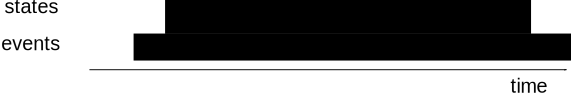
\includegraphics[width=0.75\textwidth]{images/example}
	\caption{Example of an analyzed sequence, where $e_i$ represent events for a given object (e.g., marketing campaigns directed at a given client) and $s_i$ represent the object's states (e.g., negative, neutral, or positive opinion about the analyzed company).}
	\label{fig:example}
\end{figure}

Given the above, the problem of state--changing sequential patterns can be conceptualized as follows.
Is it possible to find a subsequence of events (in this case, marketing campaigns) which will have a high probability of influencing the objects' state in a desired manner (in this case, changing the clients' opinion from a lower to a higher one).

Our proposed solution for the above--defined problem is a 3-step generic method, which can be described as follows.
In the first step, we mine the sequences of events for frequent sequential patterns, i.e., subsequences, which appear in the events dataset with a required minimal frequency.
In the second step, we map the states sequences to sequences of change.
Each state is mapped to a change indicator based on it's relation to the previous state.
A change from a lower to a higher state is encoded as ``$\uparrow$'' (\textit{up}); a change from a higher to a lower state is encoded as ``$\downarrow$'' (\textit{down}); and no change is encoded as ``$-$'' (\textit{none}).
The first state is mapped to ``$-$''.
In the third phase, we calculate the uplift measure of each sequential pattern for a given change indicator (e.g., ``$\uparrow$''), by contrasting the probability of this change appearing after a given pattern among the sequences with this pattern against the probability of this change appearing among the sequences without this pattern.
After this process, we have a list of sequential patterns with the information about their impact on a given change of state.
The whole process is summarized in Fig.~\ref{fig:concept}.

\begin{figure}[!ht]
	\centering
		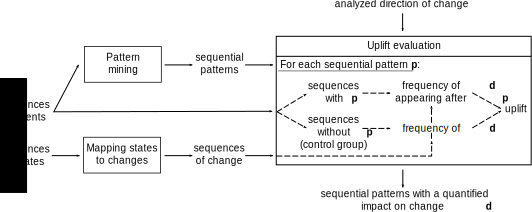
\includegraphics[width=\textwidth]{images/concept}
	\caption{Illustration of the proposed method}
	\label{fig:concept}
\end{figure}

\subsection{Formal description}
By a \textit{sequence} $s=<s_1, s_2, ..., s_n>$ we understand an ordered multi--set of \textit{elements}, where each element $s_i$ is drawn from the same set.
We distinguish two sets of sequences: sequences of events $\mathcal{S}^e$ and sequences of states $\mathcal{S}^s$, where the elements in the events sequences are drawn from the events set $\mathcal{E}$ and the elements in the states sequences are drawn from the ordered states set $\mathcal{S}$.
Each events sequence $s^e\in\mathcal{S}^e$ has a corresponding states sequence $s^{se}\in\mathcal{S}^s$ (note that this correspondence is only one--sided).
The corresponding sequences can be combined into a single sequence of events and states and there exists a total order between the elements of the combined sequences such that the order of the elements from each sequence is preserved.

We denote that a sequence $s$ \textit{contains} a pattern $p$ if $p\subseteq s$.
Given a sequence $s=<s_1,s_2,...,s_n>$, its subsequence $s'=<s_{i_1}, s_{i2}, ..., s_{i_m}>$, $1\leq m\leq n$, and an element $s_x\in s$, we say that $s_x$ appears in $s$ after $s'$ if $i_m<x\leq n$.

Given the above, our method is defined as follows.
Given a set of event sequences $\mathcal{S}^e$, a set of state sequences $\mathcal{S}^s$, a desired direction of change \textit{d}, and a minimal support threshold \textit{minsup}, first, we are mining $\mathcal{S}^e$ for sequential patterns $\mathcal{P}=\left\{p:|\{s^e\in\mathcal{S}^e:p\subseteq s^e\}|\geq\textit{minsup}\right\}$.
Next, each sequence of states $s^s\in\mathcal{S}^s$ is mapped into a sequence of changes $s^c\in\mathcal{S}^c$:
\begin{equation*}
\begin{split}
&s^c_1=-\\
&s^c_i=\begin{cases}
	\uparrow & s^s_{i-1}<s^s_i \\
	\downarrow & s^s_{i-1}>s^s_i \\
	- & otherwise
\end{cases}
\end{split}
\end{equation*}
where $i=2..|s^s|$.
The mapping preserves the correspondence relation with the events sequence and the total order of the combined elements of the events and changes sequences.
Finally, for each sequential pattern $p\in\mathcal{P}$ and a given change direction $d$, \textit{uplift} is calculated according to the following formula:
\begin{equation*}
\textit{uplift}(p,d)=P(d^p|\{s^e\in\mathcal{S}^e:p\subseteq s^e\})-P(d|\{s^e\in\mathcal{S}^e:p\not\subseteq s^e\}),
\end{equation*}
where $P(d^p|\{s^e\in\mathcal{S}^e:p\subseteq s^e\})$ denotes the probability of $d$ appearing after $p$ in sequences of events containing $p$, and $P(d|\{s^e\in\mathcal{S}^e:p\not\subseteq s^e\})$ denotes the probability of $d$ appearing in sequences of events without $p$.

\section{Experiments}
\label{sec:experiments}
\subsection{Experimental Setup}
This paper intends to evaluate the possibility of using state-changing sequential pattern mining to analyse real-world datasets, and on top of that, to assess the rightness of choice an uplift modelling to measure the actual influence of sequential pattern occurrence on the change of values of a sequence of states. Our solution was evaluated in a series of experiments using anonymised private data and publicly available datasets. We processed full datasets with different support values for each of them, using an Apriori algorithm to find sequential patterns. Also, we calculated several interestingness measures, such as support, confidence, coverage, prevalence, recall, lift, leverage, added value, Jaccard and relative risk to assess the extent of influence of a sequential pattern on the positive shift ``$\uparrow$'' (\textit{up}) in a sequence of states. Then, we compared these measures with an uplift measure. 

Experiments were prepared using software components implemented in R language. Almost all of the software components were implemented using R standard library. The exception is the component used for generation of two-element permutations of sequential candidate patterns, where we used "gtools" library. The experiments were conducted on the machine equipped with a dual-core I7-4770HQ @ 2,2 GHz processor and 16 GB of RAM.

\subsection{Datasets}
To prepare the experimental evaluation of the proposed method, we used three datasets containing sequential data. The Diabetes dataset is publicly available through the UCI Machine Learning Repository. It includes data about patients’ activity and blood sugar level measurements. A private marketing company provided the Events and Classes dataset. It contains data about marketing activity as well as the outcome of this activity. The FIFA dataset contains data about clickstream from the FIFA World Cup 98 webpage. It is publicly available on the website of SPMF – an open source data mining library.

To test the proposed solution, we amended two of the test datasets. The Diabetes dataset contains numeric attribute describing blood sugar level. We discretised this attribute into three classes, respectively describing blood sugar level as high, normal and low. Regarding the FIFA dataset, we generated the state sequence based on the original data. To each event, we assigned one of the three values describing the length of a subsequence, denoted as short, medium and long. A subsequence starts with the first element of the original sequence and finishes with the event occurrence. 

\begin{table}[htbp]
	\scriptsize
  \centering
  \caption{Characteristics of datasets}
    \begin{tabularx}{\textwidth}{l@{}R@{}R@{}R@{}R@{}R@{}R@{}}
		\toprule
	{} & \multicolumn{3}{c}{Sequence of events} & \multicolumn{3}{c}{Sequence of states} \\
        \toprule
    Dataset & \#Instances & \#Elements & Avg. len. & \#Instances & \#Elements & Avg. len.\\
		\midrule
	diabetes              &	3883	    &    20    &    7.6    &    3883    &    3    &    7.6 \\
		\midrule
	events and classes    &	4656	    &    114   &	   21.2   &    10685   &    3    &    26,5 \\
		\midrule
	fifa	                  &  20450    &  	29990  &   34.74   &    29990  &     3    &    34.74 \\
        \bottomrule
    \end{tabularx}%
  \label{tab:datasets}%
\end{table}%

\subsection{Results}


Table \ref{tab:results} presents the results of the state-changing sequential pattern mining experiments. It contains five sequential patterns with the highest uplift measure for each of the datasets. We juxtaposed these results with the others interestingness measures. Values marked in bold represent the best result of the interestingness measure in a given dataset.

We processed the diabetes dataset with \textit{minsup} = 0.4, and it allowed to find 89 sequential patterns. The values of uplift measures for these patterns were from the range \textless-0.285525302; 0.21593366\textgreater. The highest value of uplift measure has pattern \textless$\left\{\text{58}\right\}$\textgreater . Event $\{\text{58}\}$ corresponds to pre-breakfast blood glucose measurement, so it is the first activity which diabetes people do every day and also the one about which is the most difficult to forget during a daily run, what finds conformance in the high support value of this sequential pattern. Because during the day fluctuations of the blood sugar level could be high, it is highly possible that we will notice a decrease in blood sugar level, what is illustrated by the high confidence level. 

Regarding the events and classes dataset, we processed this dataset with \textit{minsup} = 0.45. As a result, we found 12 sequential patterns. The values of the uplift measure were from the range \textless 0.1412099; 0.2526986\textgreater. The highest value of uplift measure has \textless$\left\{\text{34}\right\}$,$\left\{\text{109}\right\}$\textgreater  pattern. We do not have information which marketing activity these two events describe, but the value of uplift measure allows suggesting that these consecutive activities positively influence customers’ attitude towards the brand. The support value points out that this pattern is included in around 47\% of all sequences, while the confidence value shows that occurrence of this pattern positively affected the sequence of states in 40\% of cases.

Finally, we found 5 sequential patterns with \textit{minsup}=0.4 in the FIFA dataset. The values of uplift measure were from the range \textless 0.3849705; 0.4338547\textgreater. The highest value of uplift measure has \textless$\left\{\text{90}\right\}$\textgreater pattern. We do not have information which website is described by the $\{\text{90}\}$ event in the dataset, but high value of the uplift measure suggesting that users stayed longer on the FIFA website after seeing the information contained on this website. The support value and the confidence value have values respectively of 0.4005379 and 0.9772921.

We noticed the high correlation between uplift and relative risk measures for each of analysed dataset. To understand, why does this correlation exist, it is required to take a closer look at the building of these interestingness measures. An uplift measure tries to estimate the increase of the probability of some event occurrence in a treated subpopulation over the corresponding probability when a subpopulation was not treated, whereas a relative risk is the ratio of the same probabilities. Thus, an uplift measure presents the actual change of probability, while a relative risk expresses the relative relation between probabilities.

Other measures, evaluated during our experiments, performed with a variable result. To understand this fact, it is again required to analyse differences between the construction of uplift measure and other interestingness measures used in this experimental evaluation. Uplift measure models the difference of probability of event occurrence between treated and not treated population, while measures like coverage, prevalence, recall, lift, leverage, added value and Jaccard estimate the probability of event occurrence by considering entire population. This may cause misleading results especially when the goal is to measure the change of state under some given implications.



\begin{sidewaystable}[htbp]
	\scriptsize
  \centering
  \caption{Results of state-changing mining process}
    \begin{tabularx}{\textwidth}{l@{}c@{}R@{}R@{}R@{}R@{}R@{}R@{}R@{}R@{}R@{}R@{}R@{}R@{}}
		\toprule
	{} & \multicolumn{2}{c}{Sequential pattern} & \multicolumn{11}{c}{Change measures} \\
        \toprule
    Dataset          & Seq. pattern                                                                                      & Support & Class order & Uplift      & Support   & Confidence & Coverage  & Recall    & Lift      & Leverage  & Added value & Jaccard   & Relative risk\\
		\midrule
	Diabetes         & \textless$\left\{\text{58}\right\}$\textgreater                                                         & \textbf{0.9001}                  & h \textless n \textless l   & \textbf{0.2159} & \textbf{0.8880} & 0.9866 & \textbf{0.9001}  & \textbf{0.9200} & 1.0221 & 0.1178 & 0.0213 & \textbf{0.9086} & \textbf{1.2802} \\
		\midrule
	Diabetes         & \textless$\left\{\text{58}\right\}$,$\left\{\text{33}\right\}$\textgreater                              & 0.8012                  & h \textless n \textless l   & 0.1264 & 0.7935 & 0.9904 & 0.8012  & 0.8220 & 1.0260 & 0.2170 & 0.0251 & 0.8155 & 1.1463 \\
		\midrule
	Diabetes         & \textless$\left\{\text{58}\right\}$,$\left\{\text{33}\right\}$,$\left\{\text{33}\right\}$\textgreater   & 0.7347                  & h \textless n \textless l   & 0.0941 & 0.7275 & 0.9902 & 0.7347  & 0.7537 & 1.0259 & 0.2810 & 0.0250 & 0.7481 & 1.1050 \\
		\midrule
	Diabetes         & \textless$\left\{\text{33}\right\}$\textgreater  & 0.8705 & h \textless n \textless l & 0.0922 & 0.8504 & 0.9769 & 0.8705 & 0.8810 & 1.0121 & 0.1367 & 0.0117 & 0.8630 & 1.1043 \\
		\midrule
	Diabetes         & \textless$\left\{\text{58}\right\}$,$\left\{\text{62}\right\}$,$\left\{\text{33}\right\}$\textgreater & 0.6758 & h \textless n \textless l & 0.0814 & 0.6701 & \textbf{0.9916} & 0.6758 & 0.6942 & \textbf{1.0273} & \textbf{0.3393} & \textbf{0.0264} & 0.6902 & 1.0894 \\
	    \midrule
	    \midrule
    E \& C   & $\left\{\text{34}\right\}$,$\left\{\text{109}\right\}$ & 0.4653 & a \textless b \textless c & \textbf{0.2527} & \textbf{0.1874} & \textbf{0.4028} & 0.4653 & \textbf{0.6986} & \textbf{1.5012} & 0.2779 & \textbf{0.1345} & \textbf{0.3431} & \textbf{2.6840} \\
        \midrule
    E \& C   & \textless$\left\{\text{109}\right\}$\textgreater & \textbf{0.4660} & a \textless b \textless c & 0.2520 & \textbf{0.1874} & 0.4022 & \textbf{0.4660} & 0.6986 & 1.4991 & 0.2772 & 0.1339 & 0.3427 & 2.6771 \\
        \midrule
    E \& C   & $\left\{\text{108}\right\}$,$\left\{\text{34}\right\}$ & 0.4531 & a \textless b \textless c & 0.2450 & 0.1823 & 0.4023 & 0.4531 & 0.6794 & 1.4994 & \textbf{0.2807} & 0.1340 & 0.3381 & 2.5577 \\
        \midrule
    E \& C   & \textless$\left\{\text{108}\right\}$\textgreater  & 0.4538 & a \textless b \textless c & 0.2442 & 0.1823 & 0.4017 & 0.4538 & 0.6794 & 1.4972 & 0.2799 & 0.1334 & 0.3377 & 2.5511 \\
        \midrule
    E \& C   & \textless$\left\{\text{108}\right\}$,$\left\{\text{34}\right\}$,$\left\{\text{109}\right\}$\textgreater & 0.4531 & a \textless b \textless c & 0.2436 & 0.1816 & 0.4008 & 0.4531 & 0.6770 & 1.4941 & 0.2793 & 0.1326 & 0.3365 & 2.5487 \\
	    \midrule
	    \midrule
	Fifa & \textless$\left\{\text{90}\right\}$\textgreater & 0.4005 & s \textless m \textless l & \textbf{0.4339} & 0.3914 & \textbf{0.9773} & 0.4005 & 0.5458 & \textbf{1.3626} & \textbf{0.6900} & \textbf{0.2601} & 0.5389 & \textbf{1.7984} \\
	    \midrule
    	Fifa & \textless$\left\{\text{13}\right\}$\textgreater & 0.4020 & s \textless m \textless l & 0.4277 & 0.3911 & 0.9730 & 0.4020 & 0.5453 & 1.3566 & 0.6847 & 0.2558 & 0.2558 & 1.7843 \\
    	    \midrule
    Fifa & \textless$\left\{\text{18}\right\}$\textgreater & 0.4041 & s \textless m \textless l & 0.4160 & 0.3900 & 0.9651 & 0.4041 & 0.5437 & 1.3457 & 0.6753 & 0.2479 & 0.5333 & 1.7577 \\
        \midrule
    Fifa & \textless$\left\{\text{30}\right\}$\textgreater & \textbf{0.4291} & s \textless m \textless l & 0.3950 & \textbf{0.4045} & 0.9427 & \textbf{0.4291} & \textbf{0.5641} & 1.3144 & 0.6349 & 0.2255 & \textbf{0.5454} & 1.7211 \\
        \midrule
    Fifa & \textless$\left\{\text{2}\right\}$\textgreater & 0.4003 & s \textless m \textless l & 0.3850 & 0.3795 & 0.9481 & 0.4003 & 0.5291 & 1.3219 & 0.6610 & 0.2309 & 0.5142 & 1.6836 \\
        \bottomrule
    \end{tabularx}%
  \label{tab:results}%
\end{sidewaystable}%


\section{Conclusions}
\label{sec:conclusions}
In this paper, we presented a solution to the problem of finding subsequences of events (e.g., marketing campaigns) with high probability of influencing the state of the objects targeted by these events (e.g., changing the clients’ opinion about a given brand).
We call such subsequences state--changing sequential patterns.
Our method works by mining for frequent patterns in the events sequences, mapping the states sequences to sequences encoding the changes in state, and evaluating the influence of the obtained patterns on these changes using uplift modeling.
The intuition behind this approach was to take the approach common from clinical trials and extend it to sequential data.
By experimentally testing our proposal on 3 real--world datasets we validate its usefulness for practical problems.
Furthermore, we empirically compare the employed uplift measure with 10 other measures used for sequential pattern evaluation.
The results reveal that our method allows to find sequences which could be otherwise neglected.
It also shows that uplift could be used interchangeably with relative risk, however, this was to be expected as these measures are highly related.

As the issue tackled in this paper is itself novel, the possibilities of extending this work are very broad.
As our most immediate future research focus, we plan on experimenting with introducing time constraints to the problem.
The constraints could concern both, events (e.g., restricting time gaps between events) and states (e.g., the certainty of a given object's state can decay over time until new state appears).
Moreover, we intend to create other sequential pattern evaluation measures dedicated for this specific problem.
We would also like to quantify the differences between states and include those differences in the analysis, as our current approach only registers the change in states' direction.

\subsubsection*{Acknowledgments.} This research is partly funded by the Polish National Science Center under Grant No. DEC-2015/19/B/ST6/02637.

\bibliographystyle{splncs}
\bibliography{Bibliography}

\end{document}
